\section{Using \padx{} to Query Ad Hoc Data}
\label{section:padx}

\begin{figure}
\begin{center}
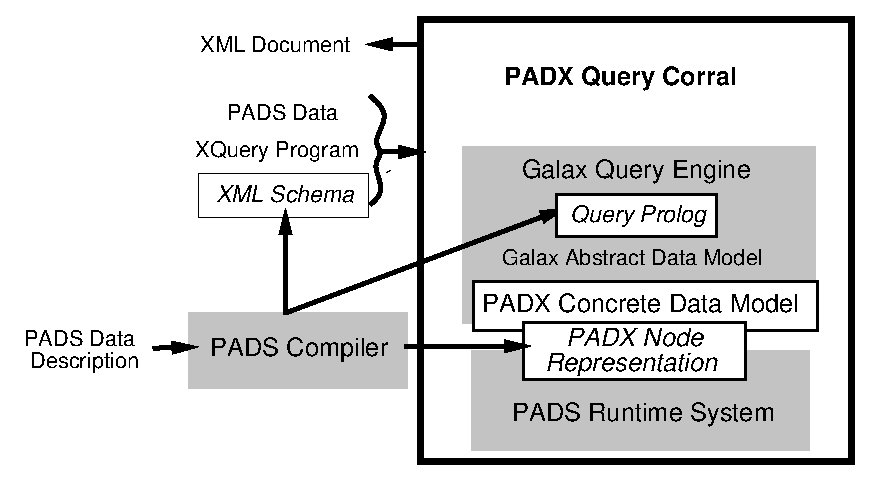
\epsfig{file=padx-arch.ps,width=0.47\textwidth}
\end{center}
\caption{\padx{} Architecture}
\label{figure:padx-arch}
\end{figure}

Figure~\ref{figure:padx-arch} depicts the \padx{} architecture.  From
a \pads{} description, the compiler generates an XML Schema
description that specifies the virtual XML view of the corresponding
\pads{} data; an XQuery prolog that imports the corresponding schema
and that associates the input data with the correct schema type; and a
type-specific library that maintains the information necessary to
support the \padx{} data model.

An instance of the \padx{} runtime system, called the ``query
corral'', consists of the \Galax{} query engine, a type-specific query
prolog, the \padx{} implementation of the \Galax{} data model, a
type-specific \padx{} library, and the \pads{} runtime system.  Note
that the resulting query corral is \emph{specialized} for a particular
\pads{} description.  From the query prolog, it imports the XML Schema
that corresponds to the underlying type-specific library, i.e., it
does permit the query writer to import an arbitrary schema.  This
restriction guarantees that the XQuery program is typed with respect
to the correct XML Schema and that the underlying data model is an
instance of the specified XML Schema.  At runtime, the query corral
takes an XQuery program and a \pads{} data source and produces the
query result in XML.  We discuss the problem of producing native
\pads{} values in Section~\ref{section:future}. 

Section~\ref{section:pads} describes the output of the \pads{}
compiler.  Here, we focus on the mapping from a description to XML
Schema and on the features of the type-specific data model.

\subsection{Virtual XML view of PADS data}

We use the fragment of the XML Schema in
Figure~\ref{figure:dibbler-schema}, which corresponds to the
description in Figure~\ref{figure:dibbler}, to illustrate the mapping
of a \pads{} description to XML Schema.
\begin{figure*}
\begin{small}
\begin{code}
<xs:schema targetNamespace="\kw{file:/example/sirius.p}"
           xmlns="file:/example/sirius.p"
           xmlns:xs="http://www.w3.org/2001/XMLSchema"
           xmlns:p="http://www.padsproj.org/pads.xsd">
<xs:import namespace = "http://www.padsproj.org/pads.xsd".../>
...
<xs:complexType name="\kw{order_header_t}">
 <xs:sequence>
  <xs:element name="\kw{order_num}"     type="\kw{p:val_Puint32}"/>
  <xs:element name="\kw{att_order_num}" type="\kw{p:val_Puint32}"/>
  <xs:element name="\kw{ord_version}"   type="\kw{p:val_Puint32}"/>
  <!-- More local element declarations -->
  <xs:element name="\kw{pd}"            type="\kw{p:PStruct_pd}" minOccurs="0"/>
 </xs:sequence>
</xs:complexType>
<!-- More complex type declarations -->
<xs:complexType name="\kw{orders_t}">
 <xs:sequence>
  <xs:element name="\kw{elt}"    type="\kw{order_t}" maxOccurs="unbounded"/>
  <xs:element name="\kw{length}" type="\kw{p:Puint32}"/>
  <xs:element name="\kw{pd}"     type="\kw{p:Parray_pd}" minOccurs="0"/>
 </xs:sequence>
</xs:complexType>
...
<xs:element name="PSource" type="summary"/>
</xs:schema>
\end{code}
\end{small}
\caption{Fragment of XML Schema for \dibbler{} \pads{} description.}
\label{figure:dibbler-schema}
\end{figure*}

``Error-aware'' mapping from PADS type system to isomorphic XML
Schema. 
\begin{small}
\begin{code}
<xs:simpleType name="Puint32">
  <xs:restriction base="xs:unsignedInt"/>
</xs:simpleType>
<xs:complexType name="\kw{val_Puint32}">
  <xs:\kw{choice}>
   <xs:element name="\kw{val}" type="\kw{p:Puint32}"/>
   <xs:element name="\kw{pd}"  type="\kw{p:Pbase_pd}"/>
  </xs:\kw{choice}>
</xs:complexType>
<xs:complexType name="\kw{Pbase_pd}">
 <xs:sequence>
   <xs:element name="\kw{pstate}"  type="\kw{p:Pflags_t}"/>
   <xs:element name="\kw{errCode}" type="\kw{p:PerrCode_t}"/>
   <xs:element name="\kw{loc}"     type="\kw{p:Ploc_t}"/>
 </xs:sequence>
</xs:complexType>
\end{code}
\end{small}

Each compound type is mapped to an XML Schema complex type.

Each base type is mapped to an XML Schema simple type.  Since the base
types do not change, the corresponding XML Schema types are defined
once in \cd{pads.xsd}, which is imported into all generated schemata. 

  One-to-one mapping
from PADS base types to XML Schema simple types.  Field in compound
types are realized as local elements in XML Schema. 

All the compound types are annotated with an optional parse-descriptor
(absent if no errors occured).  Allows users to query error
structures, which may be most important data.  Other types annotated
with corresponding fields from PADS rep, e.g., arrays have a length. 

Extra level of indirection in representation of arrays---wrap each
item in an element. 

Extra level of indirection for base types: must contain the value of
the base type and an optional parse-descriptor, if an error has
occurred. 

We don't take complete advantage of XML Schema, e.g., Penum types
could be modeled by XML Schema enumeration simple types, but currently
unsupported.

Example of query prolog. 
\begin{figure*}
\begin{small}
\begin{code}
import schema default element namespace "\kw{file:/example/sirius.p}";
declare variable \kw{$pads} as \kw{document-node(PSource)} external; 
\end{code}
\end{small}
\caption{\padx{} generated query prolog}
\label{figure:padx-query-prolog}
\end{figure*}

How to access data files:  fn:doc("pads:/example/sirius.data");

\subsection{Physical Data Model}

Part of PADX implementation are generic functions that implement data
model accessors.  PADS compiler generates type-specific functions for
walking virtual XML tree.  Relate back to type-specific library
functions mentioned in last section.

Implementation of Galax's Abstract Tree Model.

Minimum necessary to implement Galax DM:

1. Generic implementations of the DM accessors: axis::node-test(), children(),
   attributes(), name(), etc. 

2. On PADX-side, we have a virtual handle for each node in the XML
   tree--we call that a node rep.  Node rep contains pads handle
   (maintains state for PADS parser); type-specific vtable of DM
   accessors; other stuff...

   Give example of vtable for event\_t and possibly code for
   kthChildByName. 

When to actually read from PADS data?

Options: 

1. Bulk read: Materialize entire PADS representation, populate all of the PADS
reps.  Then PADX DM lazily invoked the DM accessors over this data.
Problem: if data is big, it's all sitting in memory, even if the query
only touches a fragment of the virtual XML tree.

2. Smart read: 

Many common queries permit sequential, streamed access to underlying
XML source.  Give an example.  

Smart node rep, preserves meta-data about previously read records, but
re-uses memory for reading next item.  This rep permits multiple scans
of input (semantic problem is that DM must preserve node identity),
but slowly. 

Heuristic: records are a good level of granularity to read.   Each
smart node corresponds to one record.  When next smart node is
accessed, a little meta-data is preserved: the node rep and the
records location in the file (so we can re-read it if necessary).

3. Linear read: same as smart but does not preserve meta-data.
   Does not permit multiple scans of data source. 

Put in PADX signatures for constructing a new node and accessing
kthChild. 

Something about query evaluation:
Although we have not explored custom evaluation plans 
Galax's algebra or optimizer are particularly interesting in the 
\padx{}, we expect to do so 
